\chapter{Grundlagen}

\targets{
  \item \LaTeX\ kennen lernen
  \item Aufbau von \LaTeX-Dokumente, -Befehle und Umgebungen kennen
  \item \LaTeX\ verwenden können
  \item Verstehen, wofür man \LaTeX\ einsetzen kann und wofür nicht
}

\website

\section{Was ist \LaTeX?}

\subsection{Einordnung}

\begin{Frame}{Dimensionen eines Dokumentes}
  \begin{description}
    \item[Inhalt] ist die \alert{Bedeutung} eines Textes
    \item[Struktur] ist der \alert{Aufbau} eines Textes
    \item[Form] ist das \alert{Aussehen} eines Textes
  \end{description}
\end{Frame}

\begin{Frame}{Struktur vs. Form}
  \begin{Beispiel}[Strukturelemente]
    \begin{itemize}
      \item Überschrift
      \item Listeneintrag
      \item Tabellenzelle
    \end{itemize}
  \end{Beispiel}

  \xxx

  \begin{Beispiel}[Formen]
    \begin{itemize}
      \item 16~pt, Arial, Fett, 2~em Abstand
      \item 2~cm Einzug, Bullet-Zeichen \textbullet\ am Zeilenanfang
      \item 3~cm breiter umrandeter Kasten
    \end{itemize}
  \end{Beispiel}
\end{Frame}

\begin{Frame}[fragile]{Seitenbeschreibungssprachen}
  \newcommand{\entry}[2]{\draw[maincolor, thick] (-.2,#1) -- (.2,#1) node[right] {\color{black}#2};}
  \hskip 8ex\begin{tikzpicture}
    \draw[maincolor, thick] (0,0) node[below] {\textbf{Form}} edge[<->] (0,6);
    \draw[maincolor] (0,6) node[above] {\textbf{Struktur}};
    \entry{.5}{Pixelgrafiken bzw. Paint};
    \entry{1}{Vektorgrafiken bzw. Inkscape};
    \entry{1.5}{PDF};
    \entry{2.5}{\TeX};
    \entry{3}{DTP-Tools wie z.\,B. Scribus};
    \entry{3.5}{Office Word, Writer, \ldots};
    \entry{4}{\alert{\LaTeX}};
    \entry{4.75}{HTML};
    \entry{5.5}{Outliner};
  \end{tikzpicture}
\end{Frame}

\begin{Frame}{\LaTeX}
  \textbf{\color{maincolor}Historie}
  \begin{itemize}
    \item \LaTeX\ ist ein Makropaket für das Satzsystem \TeX
      \begin{itemize}
        \item \TeX\ wurde 1977 von Donald E. Knuth enwickelt
        \item Aktuelle Version: 3.1415926 (März 2008)
      \end{itemize}
    \item \LaTeX\ wurde 1980 von Leslie Lamport entwickelt
    \item Aktuelle Version: 2011/06/27
  \end{itemize}

  \xxx
  \pause

  \inhead{Verwendung}
  \begin{itemize}
    \item Ein \LaTeX-Dokument ist ein \alert{reines Textdokument}.
    \item Das \LaTeX-Dokument enthält \alert{Inhalt und Struktur}.
    \item \LaTeX\ setzt den Inhalt und kümmert sich um \alert{gute Form}.
  \end{itemize}
\end{Frame}

\subsection{Beispiele}

\begin{Frame}{Ein \TeX-Dokument}{Quelltext \texttt{story.tex}}
  \lstinputlisting[firstline=7]{demo/story.tex}
\end{Frame}

\begin{Frame}[fragile]{Ein \TeX-Dokument}{Kompilieren}
  \begin{lstlisting}[language={},morekeywords={tex,dvips,pstopdf},gobble=4]
    tex story
    dvips story
    pstopdf story.ps
  \end{lstlisting}

  \xxx
  \pause

  \begin{onlyenv}<presentation>
    \vskip -2.3cm
    
\begin{tikzpicture}
      \draw[red,very thick] (0,0) -- (2.5cm, 2cm);
    \end{tikzpicture}
    \vskip .5cm
  \end{onlyenv}

  \begin{lstlisting}[language={},morekeywords={pdftex},gobble=4]
    pdftex story
  \end{lstlisting}
\end{Frame}

\begin{Frame}[t]{Ein \TeX-Dokument}{Quelltext \texttt{story.tex} und Dokument \texttt{story.pdf}}
  \lstinputlisting[firstline=7]{demo/story.tex}

  \begin{center}
    \includegraphics[width=10cm]{demo/story.pdf}
  \end{center}
\end{Frame}

\begin{Frame}[fragile,t]{Ein \LaTeX-Dokument}
  \inhead{\texttt{hello.tex}}
  \lstinputlisting{demo/hello.tex}

  \pause
  \xxx

  \inhead{Kompilieren}
  \begin{lstlisting}[language={},morekeywords={pdflatex},gobble=4]
    pdflatex hello
  \end{lstlisting}

  \pause
  \xxx

  \inhead{\texttt{hello.pdf}}
  \only<presentation>{\vskip-2cm\strut}
  \begin{center}
    \includegraphics[width=10cm]{demo/hello.pdf}
  \end{center}
\end{Frame}

\subsection{Installation}

\begin{Frame}[t]{Distributionen}
  \begin{Block}{Windows}
    \begin{columns}
      \column{1mm}
      \column{5cm}
      \vskip2pt\par
      
\includegraphics[width=3.5cm]{images/miktex}\\
      \column{5cm}
      installiert Pakete bei\\ erster Verwendung automatisch
    \end{columns}
    \url{www.miktex.org}
  \end{Block}

  \begin{Block}{Linux}
    \begin{columns}
      \column{1mm}
      \column{5cm}
      \vskip4pt\par
      \xdefinecolor{texlive}{RGB}{12,99,170}
      \textcolor{texlive}{\Huge\bfseries\TeX\ Live}
      \column{5cm}
      mit Installer als\\ DVD-Image verfügbar
    \end{columns}
    \vskip4pt\par
    \url{www.tug.org/texlive}
  \end{Block}

  \begin{Block}{Mac}
    \begin{columns}
      \column{1mm}
      \column{4.5cm}
      
\includegraphics[width=3.5cm]{images/mactex}
      \column{5cm}
      \TeX\ Live und Tools\\ für Mac OS
    \end{columns}
    \url{www.tug.org/mactex}
  \end{Block}
\end{Frame}

\begin{Frame}{Pakete nachinstallieren und aktualisieren}{Windows}
  \begin{figure}
    \centering
    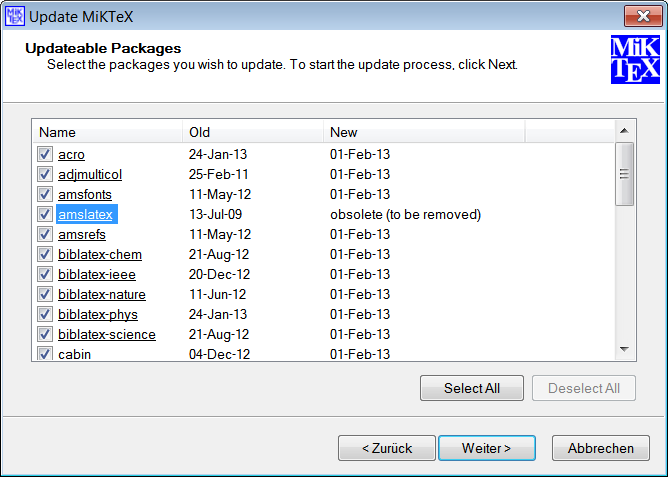
\includegraphics[width=8cm]{images/miktex-update}
    \caption{MiK\TeX\ Updater}
  \end{figure}
\end{Frame}

\begin{Frame}{Pakete nachinstallieren und aktualisieren}{Linux}
  \begin{figure}
    \centering
    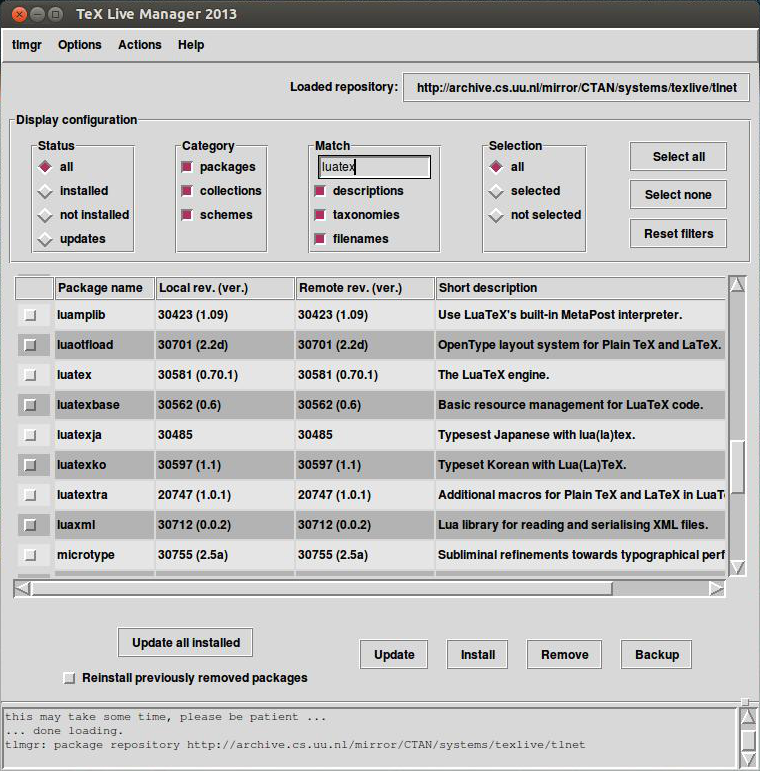
\includegraphics[width=7cm]{images/texlive-update}
    \caption{\TeX\ Live Manager}
  \end{figure}
\end{Frame}

\begin{Frame}{Pakete nachinstallieren und aktualisieren}{Mac}
  \begin{figure}
    \centering
    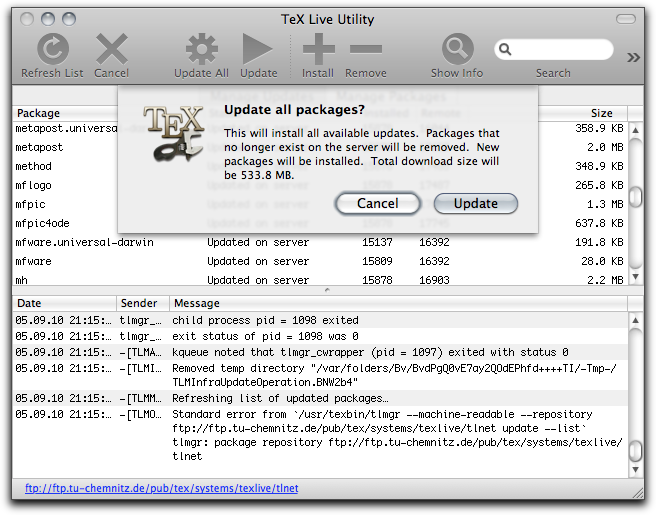
\includegraphics[width=8cm]{images/mactex-update}
    \caption{\TeX\ Live Utiliy}
  \end{figure}
\end{Frame}


\begin{Frame}[fragile]{\TeX-Live-Pakete unter Ubuntu/Debian}
  \begin{lstlisting}[gobble=4,language={},morekeywords={sudo,apt,get}]
    sudo apt-get install texlive \
      texlive-lang-german texlive-latex-extra
  \end{lstlisting}

  installiert die Pakete

  \begin{description}
    \item[texlive] vollständiges \TeX-System, 
    \item[texlive-lang-german] deutsche Sprachunterstützung und
    \item[texlive-latex-extra] viele zusätzliche \LaTeX-Pakete.
  \end{description}

  \begin{alertblock}{Manuelle Installation}
    \begin{itemize}
      \item manuelle Installation ist oft aktueller
      \item vor Ubuntu 12.10 nur \TeX\ Live 2009 verfügbar
      \item Paketmanagement mit Paket \texttt{texlive-dummy} austricksen
        (vgl. Anleitung von ubuntuusers)
    \end{itemize}
  \end{alertblock}
\end{Frame}

\begin{Frame}{Editoren und IDEs}
  \begin{Block}{Editoren}
    \begin{itemize}
      \item Notepad++ (Windows)
      \item GEdit (Linux)
      \item Sublime Text (Windows, Linux, Mac)
    \end{itemize}
  \end{Block}

  \pause

  \begin{Block}{IDEs}
    \begin{itemize}
      \item \TeX works
        \begin{itemize}
          \item in MiK\TeX, \TeX\ Live und Mac\TeX\ enthalten
        \end{itemize}
      \item \TeX Shop
        \begin{itemize}
          \item Apple Design Award 2002
          \item in Mac\TeX\ enthalten
        \end{itemize}
      \item Kile (Linux)
      %\item Texmaker (Windows, Linux, Mac)
      \item TeXstudio (Windows, Linux, Mac)
      %\item \TeX nicCenter (Windows)
    \end{itemize}
  \end{Block}
\end{Frame}

\section{\LaTeX\ verwenden}

\subsection{Aufbau und Präambel}

\begin{Frame}[fragile]{Befehle}
  \begin{Definition}[Befehl]
    \begin{lstlisting}[gobble=6,style=block,morekeywords={commandname}]
      \commandname*[opt]{arg1}{arg2}
    \end{lstlisting}

    \begin{tabular}{rl}
      \lstinline[morekeywords={commandname}]-commandname- & Name des Befehls \\
      \lstinline-*- & optionaler Schalter \\
      \lstinline-[opt]- & optionaler Parameter \\
      \lstinline-{arg1}- & Parameter
    \end{tabular}
  \end{Definition}

  \xxx

  \begin{Beispiel}[Befehl]
    \begin{lstlisting}[gobble=6,style=block]
      \section[Kurzform]{Überschrift}
      \section*{noch eine Überschrift}
    \end{lstlisting}
  \end{Beispiel}
\end{Frame}

\begin{Frame}[fragile]{Umgebungen}
  \begin{Definition}[Umgebung]
    \begin{lstlisting}[gobble=6,style=block]
      \begin{envname}[opt]{arg1}{arg2}
        Inhalt
      \end{envname}
    \end{lstlisting}

    \begin{tabular}{rl}
      \lstinline-envname- & Name der Umgebunng \\
      \lstinline-Inhalt- & Inhalt der Umgebung
    \end{tabular}
  \end{Definition}

  \xxx

  \begin{Beispiel}[Umgebung]
    \begin{lstlisting}[gobble=6,style=block]
      \begin{center}
        Ich bin zentriert.
      \end{center}
    \end{lstlisting}
  \end{Beispiel}
\end{Frame}

\begin{Frame}[fragile]{Aufbau eines Dokuments}
  \begin{tikzpicture}[%
      auto,
      every edge/.style={
        draw,
        decorate,
        decoration=brace,
        maincolor,
        very thick
      }
    ]
    \node[text width=\textwidth, anchor=south] (tex) {
      \begin{lstlisting}[gobble=8]
        \documentclass{scrartcl}

        \usepackage[babel]{ngerman}
        \usepackage[utf8]{inputenc}
        \usepackage[T1]{fontenc}

        \title{Hallo Welt}
        \author{Malte Schmitz}

        \begin{document}
          \maketitle

          \section{erster Abschnitt}
          Hier beginnt's \ldots
        \end{document}
      \end{lstlisting}
    };

    \pause
    \draw
      (1,5.5) edge node {Dokumentenklasse} (1,5.2);
    \pause
    \draw
      (3,4.9) edge node {Präambel} (3,2.8)
      (0,4.8) edge node {\shortstack{Pakete\\laden}} (0,3.8)
      (0,3.5) edge node {Einstellungen} (0,2.8);
    \pause
    \draw
      (1,2.2) edge node {Dokumentenkörper} (1,.8);
  \end{tikzpicture}
\end{Frame}

\begin{Frame}[fragile]{typische Präambel}{Dokumentenklasse}
  \lstinline-\documentclass{scrartcl}-\\
  kurzer Artikel

  \xxx

  \lstinline-\documentclass{scrreprt}-\\
  Bericht mit Titelseite und Kapiteln

  \xxx

  \lstinline-\documentclass{scrbook}-\\
  doppelseitiges Buch mit Teilen, Kapiteln und Kopfzeile

  \xxx

  \begin{alertblock}{amerikanische Dokumentenklassen}
    Wir verwenden die deutschen Dokumentenklassen aus KOMA-Script statt der 
    amerikanischen \lstinline-article-, \lstinline-report- und \lstinline-book-.
  \end{alertblock}
\end{Frame}

\begin{Frame}[fragile]{typische Präambel}{KOMA-Script-Optionen}
  \begin{lstlisting}[gobble=4]
    \documentclass[
      parskip=full,
      % full - Absätze haben großen Abstand
      % half - Absätze haben kleinen Abstand
      % off - Absätze haben Einzug (default)
      fontsize=12pt,
      % Grunschriftgröße (10pt default)
      headings=small,
      % small - kleine Überschriften
      % normal - normale Überschriften (default)
      % big - große Überschriften
      paper=a5,
      % Papierformat (a4 default)
      pagesize=auto
      % Papierformat auch für PDF verwenden
    ]{scrartcl}
  \end{lstlisting}
\end{Frame}

\begin{Frame}[fragile]{typische Präambel}{Pakete}
  \lstset{
    backgroundcolor={},
    frame=no,
    gobble=4,
    aboveskip=3ex,
    belowskip=0pt
  }
  \begin{lstlisting}
    \usepackage[babel]{ngerman}
  \end{lstlisting}
  Deutsche Silbentrennung und deutsche Übersetzung
  \begin{lstlisting}
    \usepackage[utf8]{inputenc}
  \end{lstlisting}
  UTF-8 als Zeichenkodierung verwenden
  \begin{lstlisting}
    \usepackage[T1]{fontenc}
    \usepackage{lmodern}
  \end{lstlisting}
  schönere Schriftarten
  \begin{lstlisting}
    \usepackage[breaklinks=true, pdfborder={0 0 0},
                pdfhighlight={/N}]{hyperref}
  \end{lstlisting}
  bessere Unterstützung der PDF-Ausgabe
\end{Frame}

\subsection{Auszeichnungen}

\begin{Frame}[fragile]{Absätze}
  \begin{Block}{Absatz}
    \begin{itemize}
      \item leere Zeile in der Eingabe
      \item Aussehen je nach Einstellungen (\lstinline-parskip-, \ldots)
    \end{itemize}
  \end{Block}

  \begin{Block}{manuelle Umbrüche}
    \begin{itemize}
      \item braucht man nicht
      \item machen das Dokument kaputt
      \item Zeilenumbruch: \lstinline-\\-
      \item Seitenumbruch: \lstinline-\newpage-
    \end{itemize}
  \end{Block}
\end{Frame}

\begin{Frame}[fragile]{Ausrichtung}
  \newcommand{\lorem}{\textcolor{black!40}{Auch in der zweiten Zeile. Lorem ipsum dolor sit amet, consectetur, adipisci velit, \ldots}}

  \begin{minipage}{\textwidth}
    Ohne Umgebung wird Text immer im Blocksatz gesetzt.
    \lorem
  \end{minipage}

  \xxx

  \begin{center}
    Text in der Umgebung \lstinline-center- wird \alert{zentriert}
    gesetzt.
    \lorem
  \end{center}

  \xxx

  \begin{flushleft}
    Text in der Umgebung \lstinline-flushleft- wird als
    \alert{linksbündiger Flattersatz} gesetzt.
    \lorem
  \end{flushleft}

  \xxx

  \begin{flushright}
    Text in der Umgebung \lstinline-flushright- wird als
    \alert{rechtsbündiger Flattersatz} gesetzt.
    \lorem
  \end{flushright}
\end{Frame}

\begin{Frame}[fragile]{Auszeichnungen}
  \begin{Block}{Text hervorheben}
    \begin{itemize}
      \item \lstinline-\emph{hervor}- hebt \emph{hervor}
      \item \lstinline-\textit{kursiv}- setzt \textit{kursiv}
      \item \lstinline-\textsl{schräg}- setzt \textsl{schräg}
      \item \lstinline-\textsc{in Kapitälchen}- setzt \textsc{in Kapitälchen}
      \item \lstinline-\textbf{fett}- setzt \textbf{fett} \uncover<2>{\alert{(nicht!)}}
      \item \lstinline-\underline{unterstrichen}- setzt \underline{unterstrichen} \uncover<2>{\alert{(nicht!)}}
    \end{itemize}
  \end{Block}
  
  \begin{Block}{Schriftarten}
    \begin{itemize}
      \item \lstinline-\textsf{serifenlos}- setzt \textsf{serifenlos}
      \item \lstinline-\textrm{mit Serifen}- setzt \textrm{mit Serifen}
      \item \lstinline-\texttt{nichtproportional}- setzt \texttt{nichtproportional}
    \end{itemize}
  \end{Block}
\end{Frame}

\begin{Frame}[fragile]{Schriftgröße}
  \begin{itemize}
    \item \lstinline-{\tiny winzig}- setzt {\tiny winzig}
    \item \lstinline-{\scriptsize in Indexgröße}- setzt {\scriptsize in Indexgröße}
    \item \lstinline-{\footnotesize in Fußzeilengröße}- setzt {\footnotesize in Fußzeilengröße}
    \item \lstinline-{\small klein}- setzt {\small klein}
    \item \lstinline-{\normalsize in Normalgröße}- setzt {\normalsize in Normalgröße}
    \item \lstinline-{\large groß}- setzt {\large groß}
    \item \lstinline-{\Large größer}- setzt {\Large größer}
    \item \lstinline-{\LARGE am größten}- setzt {\LARGE am größten}
    \item \lstinline-{\huge riesig}- setzt {\huge riesig}
    \item \lstinline-{\Huge riesiger}- setzt {\Huge riesiger}
  \end{itemize}
\end{Frame}

\begin{Frame}[fragile]{Abkürzungen}
  \begin{Block}{Mehrgliedrige Abkürzungen}
    \begin{tabular}{rll}
      nicht: & \lstinline-z.B.- & z.B. \\
      auch nicht: & \lstinline-z.~B.- & z.~B. \\
      sondern: & \lstinline-z.\,B.- & z.\,B. \\
    \end{tabular}
  \end{Block}
  
  \begin{Block}{Trennung von Abkürzungen}
    \begin{itemize}
      \item Abkürzungen nicht trennen
      \item Maß- und Währungszeichen nicht von der Zahl trennen
      \item geschütztes Leerzeichen \lstinline-~- verwenden\\
        Beispiele: \lstinline-Seite~5, 4~km, S.~5~ff.-
    \end{itemize}
  \end{Block}
\end{Frame}

\begin{Frame}[fragile]{Anführungszeichen}
  \begin{alertblock}{Verwendung}
    Anführungszeichen sind nur für \alert{wörtliche Zitate}.
  \end{alertblock}
  
  \begin{Block}{In der Präambel}
    \begin{lstlisting}[gobble=6,style=block]
      \usepackage[german=guillemets]{csquotes}
      %      oder german=quotes
      %      oder english=british oder english=american
    \end{lstlisting}
  \end{Block}

  \begin{lstlisting}[gobble=4]
    Hans sagt: \enquote{Er rief: \enquote{Franz' Auto!}}
  \end{lstlisting}

  Hans sagt: \enquote{Er rief: \enquote{Franz' Auto!}}
\end{Frame}

\begin{Frame}[fragile]{Binde- und sonstige Striche}
  \begin{itemize}
    \item Bindestrich\newline
      \lstinline|SOS-Ruf|\newline
      SOS-Ruf
    \item deutscher Gedankenstrich mit Leerzeichen\newline
      \lstinline|Er kam -- und ging gleich wieder.|\newline
      Er kam -- und ging gleich wieder.
    \item britischer Gedankenstrich ohne Leerzeichen\newline
      \lstinline|He came---and went.|\newline
      He came---and went.
    \item Gedankenstrich für Bereiche ohne Leerzeichen\newline
      \lstinline|Das Buch darf 10--12 Euro kosten.|\newline
      Das Buch darf 10--12 Euro kosten.
    \item Minuszeichen als binärer und unärer Operator\newline
      \lstinline|$2-4=-2$ (nicht -2)|\newline
      $2-4=-2$ (nicht -2)
      \only<article>{
        \newline Als binärer Operator wird das Minuszeichen mit einem kleinen Abstand gesetzt.
        Als unärer Operator wird das Minuszeichen als Vorzeichen ohne Abstand gesetzt.
        \LaTeX\ übernimmt dies automatisch.
      }
  \end{itemize}
\end{Frame}

\subsection{Formelsatz}

\begin{Frame}[fragile]{Formelsatz in der Matheumgebung}
  \begin{Block}{In der Präambel}
    \begin{lstlisting}[gobble=6,style=block]
      \usepackage{amsmath}
      \usepackage{amssymb}
    \end{lstlisting}
  \end{Block}
  
  \begin{itemize}
    \item in normalen Text: \lstinline-$x^y$- erzeugt $x^y$
    \item abgesetzt: \lstinline-\[ x^3 \]- erzeugt
      \[ x^3 \]
    \item mehrzeilig: \lstinline-align-, ausgerichtet an \lstinline-&-, neue Zeile mit \lstinline-\\- 
      \begin{lstlisting}[gobble=8]
        \begin{align} % ohne Nummerierung mit align*
          f(x) &= x^3 \\
               &= x \cdot x \cdot x
        \end{align}
      \end{lstlisting}
      \begin{align}
        f(x) &= x^3 \\
             &= x \cdot x \cdot x
      \end{align}
  \end{itemize}
\end{Frame}

\begin{Frame}[fragile]{Beispiele zum Formelsatz}
  \begin{columns}
    \column{5cm}
      \begin{lstlisting}[gobble=8]
        \alpha^{22} + \beta_{12}
          = \gamma^2_a
      \end{lstlisting}
    \column{4cm}
      $\displaystyle\displaystyle\alpha^{22} + \beta_{12} = \gamma^2_a$
  \end{columns}

  \pause

  \begin{columns}
    \column{5cm}
      \begin{lstlisting}[gobble=8]
        \sum_{i=1}^{n} i =
          \frac{n(n+1)}{2}
      \end{lstlisting}
    \column{4cm}
      $\displaystyle\sum_{i=1}^n i = \frac{n(n+1)}{2}$
  \end{columns}

  \pause

  \begin{columns}
    \column{5cm}
      \begin{lstlisting}[gobble=8]
        \sqrt{x^{4}} = x^{2}
      \end{lstlisting}
    \column{4cm}
      $\displaystyle\sqrt{x^4} = x^2$
  \end{columns}

  \pause

  \begin{columns}
    \column{5cm}
      \begin{lstlisting}[gobble=8]
        \lim_{n\to\infty}
          \frac{1}{n^{2}} = 0
      \end{lstlisting}
    \column{4cm}
      $\displaystyle\lim_{n\to\infty} \frac{1}{n^2} = 0$
  \end{columns}
  
  \pause

  \begin{columns}
    \column{5cm}
      \begin{lstlisting}[gobble=8]
        \int_{-1}^{2}
          x\,\mathrm{d}x = \left[
            \frac{1}{2}x^{2}
          \right]_{1}^{2}
      \end{lstlisting}
    \column{4cm}
      $\displaystyle\int_{-1}^{2} x\,\mathrm{d}x=\left[ \frac{1}{2}x^2 \right]_1^2$
  \end{columns}
\end{Frame}

\subsection{Listen, Tabellen, Grafiken}

\begin{Frame}[fragile]{Listen}
  \begin{columns}
    \column{5cm}
      \begin{lstlisting}[gobble=8]
        \begin{itemize}
          \item Apfel
            \begin{itemize}
              \item Holsteiner Cox
              \item Braeburn
            \end{itemize}
          \item Birne
        \end{itemize}
      \end{lstlisting}
    \column{4cm}
      \begin{itemize}
        \item Apfel
          \begin{itemize}
            \item Holsteiner Cox
            \item Braeburn
          \end{itemize}
        \item Birne
      \end{itemize}
  \end{columns}
  
  \begin{columns}
    \column{5cm}
      \begin{lstlisting}[gobble=8]
        \begin{enumerate}
          \item Apfel
            \begin{enumerate}
              \item Holsteiner Cox
              \item Braeburn
            \end{enumerate}
          \item Birne
        \end{enumerate}
      \end{lstlisting}
    \column{4cm}
      \begin{enumerate}
        \item Apfel
          \begin{enumerate}
            \item Holsteiner Cox
            \item Braeburn
          \end{enumerate}
        \item Birne
      \end{enumerate}
  \end{columns}
\end{Frame}

\begin{Frame}[fragile]{Listen}{Definitionslisten}
  \begin{lstlisting}[gobble=4]
    \begin{description}
      \item[Das Schlagwort] steht am Anfang einer Zeile und
        wird hervorgehoben, während der zugehörige
      \item[Text] dahinter in normaler Schrift erscheint.
    \end{description}
  \end{lstlisting}

  \begin{description}
    \item[Das Schlagwort] steht am Anfang einer Zeile und wird
      hervorgehoben, während der zugehörige
    \item[Text] dahinter in normaler Schrift erscheint.
  \end{description}
\end{Frame}

\begin{Frame}[fragile]{Tabellen}
  \begin{lstlisting}[gobble=4]
    \begin{tabular}{l|lr}
      \textbf{Jahr} & \textbf{Prozessor} & \textbf{MHz} \\
      \hline
      1975 & 6502 (C64) & 1 \\
      1985 & 80386 & 16 \\
      2005 & Pentium 4 & 2\,800 \\
      2030 & Phoenix 3 & 7\,320\,000
    \end{tabular}
  \end{lstlisting}

  \begin{center}
    \begin{tabular}{l|lr}
      \textbf{Jahr} & \textbf{Prozessor} & \textbf{MHz} \\
      \hline
      1975 & 6502 (C64) & 1 \\
      1985 & 80386 & 16 \\
      2005 & Pentium 4 & 2\,800 \\
      2030 & Phoenix 3 & 7\,320\,000
    \end{tabular}
  \end{center}
\end{Frame}

\begin{Frame}[fragile]{Grafiken}
  \begin{columns}
    \column{5cm}
      \begin{lstlisting}[gobble=8]
        \includegraphics%
          [width=3.5cm]{miktex}
      \end{lstlisting}
    \column{4cm}
      
\includegraphics[width=3.5cm]{images/miktex}
  \end{columns}

  \begin{columns}
    \column{5cm}
      \begin{lstlisting}[gobble=8]
        \includegraphics%
          [width=3.5cm,%
           angle=20]{miktex}
      \end{lstlisting}
    \column{4cm}
      
\includegraphics[width=3.5cm,angle=20]{images/miktex}
  \end{columns}

  \begin{columns}
    \column{5cm}
      \begin{lstlisting}[gobble=8]
        \includegraphics%
          [width=3.5cm,%
           trim=3cm 5mm 4cm 12mm,%
           clip=true]{miktex}
      \end{lstlisting}
    \column{4cm}
      
\includegraphics[width=3.5cm,trim=3cm 5mm 4cm 12mm,clip=true]{images/miktex}
  \end{columns}
  schneidet links 3\,cm, unten 5\,mm,\\ rechts 4\,cm und oben 12\,mm ab
\end{Frame}

\section{Verzeichnisse und Verweise}

\subsection{Struktur des Dokuments}

\begin{Frame}[fragile]{Inhaltsverzeichnis}
  \begin{Block}{Strukturbefehle}
    \begin{itemize}
      \item \lstinline-\part{name}- für Teile (nur in Büchern)
      \item \lstinline-\chapter{name}- für Kapitel (nicht in Artikeln)
      \item \lstinline-\section{name}- für Abschnitte
      \item \lstinline-\subsection{name}- für Unterabschnitte
      \item \lstinline-\subsubsection{name}- für Unterunterabschnitte
      \item \lstinline-\paragraph{name}- für Absätze
    \end{itemize}
  \end{Block}

  \begin{lstlisting}[gobble=4]
    \tableofcontents
  \end{lstlisting}
  setzt das zugehörige Inhaltsverzeichnis.
\end{Frame}

\begin{Frame}[fragile]{Titelseite}{automatisch}
  \begin{Block}{In der Präambel}
    \begin{lstlisting}[gobble=6,style=block]
       \title{Meine Arbeit}
       \author{Malte Schmitz}
       \date{September 2013} % aktuelles Datum bei Auslassung
    \end{lstlisting}
  \end{Block}

  \begin{Block}{Am Anfang des Dokuments}
    \begin{lstlisting}[gobble=6,style=block]
      \maketitle
    \end{lstlisting}
  \end{Block}
\end{Frame}

\begin{Frame}[fragile]{Titelseite}{manuell}
  \begin{lstlisting}[gobble=4]
    \begin{titlepage}
      \begin{center}
        \textsf{\textbf{\Huge Meine Arbeit}}

        \textsf{\Large Malte Schmitz}
      \end{center}
    \end{titlepage}
  \end{lstlisting}
\end{Frame}

\subsection{Abbildungen}

\begin{Frame}[fragile]{Abbildungen und Tabellen}
  \begin{Block}{Fließumgebungen}
    Abbildungen und Tabellen werden\\
    automatisch im Dokument positioniert.
  \end{Block}

  \begin{lstlisting}[gobble=4]
    \begin{figure}
      
\includegraphics[width=3.5cm]{miktex}
      \caption{Mik\TeX-Logo}
    \end{figure}
  \end{lstlisting}

  \begin{lstlisting}[gobble=4]
    \begin{table}
      \begin{tabular}{ll}
        Umgebung & Verwendung \\
        table & Tabellen \\
        figure & Abbildungen
      \end{tabular}
      \caption{Verwendung von Abbildungen und Tabellen}
    \end{table}
  \end{lstlisting}
\end{Frame}

\begin{Frame}[fragile]{Positionierungshinweise}
  \begin{lstlisting}[gobble=4]
    \begin{figure}[htb]
      \centering
      
\includegraphics[width=3.5cm]{miktex}
      \caption{Mik\TeX-Logo}
    \end{figure}
  \end{lstlisting}

  \xxx

  Element platzieren
  \begin{description}
    \item[h] an Position im Quelltext
    \item[b] am Ende einer Seite
    \item[t] am Anfang einer Seite
    \item[p] auf einer eigenen Abbildungsseite
    \item[!] \LaTeX s Bewertung der Platzierung abschalten
  \end{description}
\end{Frame}

\begin{Frame}[fragile]{Verzeichnisse}
  \begin{Block}{Inhaltsverzeichnis}
    \begin{lstlisting}[gobble=6,style=block]
      \tableofcontents
    \end{lstlisting}
  \end{Block}

  \begin{Block}{Abbildungsverzeichnis}
    \begin{lstlisting}[gobble=6,style=block]
      \listoffigures
    \end{lstlisting}
  \end{Block}

  \begin{Block}{Tabellenverzeichnis}
    \begin{lstlisting}[gobble=6,style=block]
      \listoftables
    \end{lstlisting}
  \end{Block}

  \xxx

  \begin{alertblock}{Warnung}
    Welchen Nutzen haben Abbildungs- und Tabellenverzeichnis?
  \end{alertblock}
\end{Frame}

\subsection{Verweise}

\begin{Frame}[fragile]{Verweise}
  \begin{itemize}
    \item \alert{Nach} dem Strukturbefehl Label angeben
      \begin{lstlisting}[gobble=8]
        \section{Verzeichnisse und Verweise}
        \label{sec-verweise}
        % ...
        \begin{figure}
          
\includegraphics[width=3.5cm]{miktex}
          \caption{Mik\TeX-Logo}
          \label{fig-miktex}
        \end{figure}
      \end{lstlisting}
     \item Label referenzieren
       \begin{lstlisting}[gobble=8]
         \ldots Mik\TeX-Logo auf \autoref{fig-miktex}
         in \autoref{sec-verweise} \ldots
       \end{lstlisting}
       \ldots Mik\TeX-Logo auf Abbildung 5 in Abschnitt 3.2 \ldots
  \end{itemize}
\end{Frame}

\newcommand{\icon}[1]{%
  \tikz\draw[very thick, line join=round]
    (-.5,.5) -- ++(.7,0) -- ++(.3,-.3) --
    ++(-.3,0) -- ++(0,.3) -- ++(.3,-.3) -- ++(0,-.8) -- ++(-1,0) -- cycle
    ++ (0,-.3) node[fill, text=white,
      inner sep=2pt, minimum width=8mm, anchor=center] {#1}
    ++ (.1,-.3) -- ++(.8,0) -- ++(0,-.1)
    -- ++(-.8,0) -- ++(0,-.1)
    -- ++(.8,0) -- ++(0,-.1)
    -- ++(-.8,0) -- ++(0,-.1)
    -- ++(.8,0);
  }

\begin{Frame}{Mehrfach kompilieren hilft}{Rerun to get cross-references right.}
  \begin{center}
    \begin{tikzpicture}[on grid, node distance=18mm and 35mm]
      \node[examplecolor] (tex) {\icon{TEX}};
      \uncover<2->{
        \node[right=of tex, node font=\rmfamily\Large\bfseries]
          (pdfTeX1) {pdf\TeX};
      }
      \uncover<3>{
        \node[right=of pdfTeX1, maincolor] (pdf1) {\icon{PDF}};
        \node[below=of pdfTeX1, xshift=1cm] (log1) {\icon{LOG}};
      }
      \uncover<4->{
        \node[right=of pdfTeX1, maincolor!30] (pdf1) {\icon{PDF}};
        \node[below=of pdfTeX1, xshift=1cm, black!30] (log1) {\icon{LOG}};
      }
      \uncover<3->{
        \node[below=of pdfTeX1, xshift=-1cm, blue] (aux1) {\icon{AUX}};
      }
      \uncover<4->{
        \node[below=of aux1, xshift=1cm, node font=\rmfamily\Large\bfseries]
          (pdfTeX2) {pdf\TeX};
      }
      \uncover<5>{
        \node[right=of pdfTeX2, maincolor] (pdf2) {\icon{PDF}};
        \node[below=of pdfTeX2, xshift=1cm] (log2) {\icon{LOG}};
        \node[below=of pdfTeX2, xshift=-1cm, blue] (aux2) {\icon{AUX}};
      }
      \only<2->{
        \draw[very thick]
          (tex) edge[->] (pdfTeX1);
      }
      \only<3->{
        \draw[very thick]
          (pdfTeX1) edge[->] (aux1);
      }
      \only<3>{
        \draw[very thick]
          (pdfTeX1) edge[->] (pdf1)
                    edge[->] (log1);
      }
      \only<4->{
        \draw[very thick, black!30]
          (pdfTeX1) edge[->] (pdf1)
                    edge[->] (log1);
      }
      \only<4->{
        \draw[very thick]
          (aux1) edge[->] (pdfTeX2);
        \draw[->, very thick] (tex.south) ++ (.2,0) |- (pdfTeX2);
      }
      \only<5->{
        \draw[very thick]
          (pdfTeX2) edge[->] (pdf2)
                    edge[->] (aux2)
                    edge[->] (log2);
      }
    \end{tikzpicture}
  \end{center}
\end{Frame}

\section*{Zusammenfassung}

\begin{frame}{Zusammenfassung}
  \begin{enumerate}
    \item Das \alert{\LaTeX-Dokument} enthält \alert{Inhalt und Struktur}.
    \item \LaTeX\ setzt ein druckfertiges \alert{PDF-Dokument} und kümmert sich dabei um die \alert{gute Form}.
    \item Es ist schwierig, \alert{neue Layouts} zu erzeugen.
    \item Ein \LaTeX-Dokument besteht aus \alert{Dokumentenklasse}, \alert{Präambel} und \alert{Dokumentenkörper}.
    \item Wir haben \alert{Auszeichnungen}, \alert{Formelsatz}, \alert{Listen}, \alert{Tabellen}, \alert{Abbildungen}, \alert{Verzeichnisse} und \alert{Verweise} kennen gelernt.
  \end{enumerate}
\end{frame}

\begin{Frame}[fragile]{Zum Weiterlesen}
  \begin{thebibliography}{10}
    \bibitem{Kopka}
      Helmut Kopka.
      \newblock \emph{LATEX, Band 1: Einführung},
      \newblock Addison-Wesley, März 2002.
    \bibitem{Braune}
      Klaus Braune, Joachim und Marion Lammarsch.
      \newblock \emph{\LaTeX: Basissystem, Layout, Formelsatz},
      \newblock Addison-Wesley, Mai 2006.
    \bibitem{Struckmann}
      Werner Struckmann.
      \newblock \emph{Einige typographische Grundregeln und ihre Umsetzung in \LaTeX},
      \newblock \alt<presentation>{\href{http://www2.informatik.hu-berlin.de/sv/lehre/typographie.pdf}{\texttt{typographie.pdf}}}{\url{http://www2.informatik.hu-berlin.de/sv/lehre/typographie.pdf}}, September 2007.
    \bibitem{Kohm}
      Markus Kohm, Jens-Uwe-Morawski.
      \newblock \emph{KOMA-Script},
      \newblock \alt<presentation>{\href{http://mirrors.ctan.org/macros/latex/contrib/koma-script/doc/scrguide.pdf}{\texttt{scrguide.pdf}}}{\url{http://mirrors.ctan.org/macros/latex/contrib/koma-script/doc/scrguide.pdf}}, Juli 2012.
  \end{thebibliography}
\end{Frame}